% Nikolay Dubina 2021
\documentclass[t,pdf]{beamer}
\usetheme{CambridgeUS}

\usepackage{minted}
\usepackage{mdframed}
\usepackage{csquotes}

\setminted[sql]{fontsize=\fontsize{8}{8}}

\global\mdfdefinestyle{codeframe}{
    backgroundcolor=black!10, 
    rightline=false,
    leftline=false,
}

\AtBeginSection[]{
  \begin{frame}
  \vfill
  \centering
  \begin{beamercolorbox}[sep=8pt,center,shadow=true,rounded=true]{title}
    \usebeamerfont{title}\insertsectionhead\par
  \end{beamercolorbox}
  \vfill
  \end{frame}
}

\title[SQL Foundations]{SQL Foundations}
\subtitle{Overview of SQL and database technologies}
\author{github.com/nikolaydubina}
%\institute{Your Faculty/Department}
\date{2021}

\begin{document}

\begin{frame}
  \titlepage
\end{frame}

\begin{frame}{Outline}
  \tableofcontents
\end{frame}

\begin{frame}{About me}

\begin{itemize}
    \item Enswers, Korea — content search, backend, C++
    \item Facebook Internal Tools, USA — fullstack, Hack, Python
    \item Facebook Catalog, UK — fullstack, machine learning, Hack, Python
    \item Balancehero, Korea — data engineering, modeling, backend, Python
    \item FoundingSocieties, Singapore — backend, Go
    \item Foodpanda, Singapore — backend, Go
\end{itemize}

\end{frame}

\section{Introduction}

\begin{frame}{SQL, what is it?}
Structured Query Language
\end{frame}

\begin{frame}{Why would you need any database?}
\begin{itemize}
    \item language agnostic storage (e.g. can call from Java, Python, C++)
    \item high performance (search, modifications)
    \item fault tolerant (backups, replication)
    \item durable (will last many years)
    \item many years in operation by countless companies
    \item scales well with more data, more complex data, more traffic
\end{itemize}
\end{frame}

\begin{frame}{Why would you need SQL?}
\begin{itemize}
    \item universal — learn once and use in any project, company, language
    \item expressive — used by analysts and backend engineers
    \item many years in operation — used since 1970, origins of software
    \item high-level — decouples how to compute from what to compute
\end{itemize}
\end{frame}

\section{Language}

\begin{frame}{Basic example}
Basic query, which is typical for OLTP, business logic, debugging looks like this

\begin{mdframed}[style=codeframe]\inputminted{sql}{basic.sql}\end{mdframed}
\end{frame}

\begin{frame}{Aggregations}
Multiple rows from database can be aggregated into one and aggregate functions applied to columns. Only groups with conditions will be selected. Ordering is applied.

\begin{mdframed}[style=codeframe]\inputminted{sql}{aggregations.sql}\end{mdframed}
\end{frame}

\begin{frame}{Transactions}
For certain cases it is very important to guarantee that multiple updates happen together not not happen at all.

\begin{mdframed}[style=codeframe]\inputminted{sql}{transactions.sql}\end{mdframed}
\end{frame}

\begin{frame}{Joins, Unions}
You can access multiple data sets and join them together into a new one. 
Data can reside in different tables, databases, or views.

\begin{mdframed}[style=codeframe]\inputminted{sql}{joins.sql}\end{mdframed}
\end{frame}

\begin{frame}{Windows}
You can make aggregate queries and access columns in ordered rows.

\begin{mdframed}[style=codeframe]\inputminted{sql}{windows.sql}\end{mdframed}
\end{frame}

\begin{frame}{Unstructured data}
Many engines support unstructured data like JSON with UDFs. You can extract data, create new one, index for search. Bellow is GCP BigQuery.

\begin{mdframed}[style=codeframe]\inputminted{sql}{unstructured.sql}\end{mdframed}
\end{frame}

\begin{frame}{Geospatial queries}
Many databases allow geospatial queries using latitude, longtitude, or even free form address text\footnote{address is processed into index-able representation first}. Bellow is AWS Athena.

\begin{mdframed}[style=codeframe]\inputminted{sql}{athena-geo.sql}\end{mdframed}
\end{frame}

\begin{frame}{Functions}
Many more functions are provided and if something is missing it can be added into engine itself.

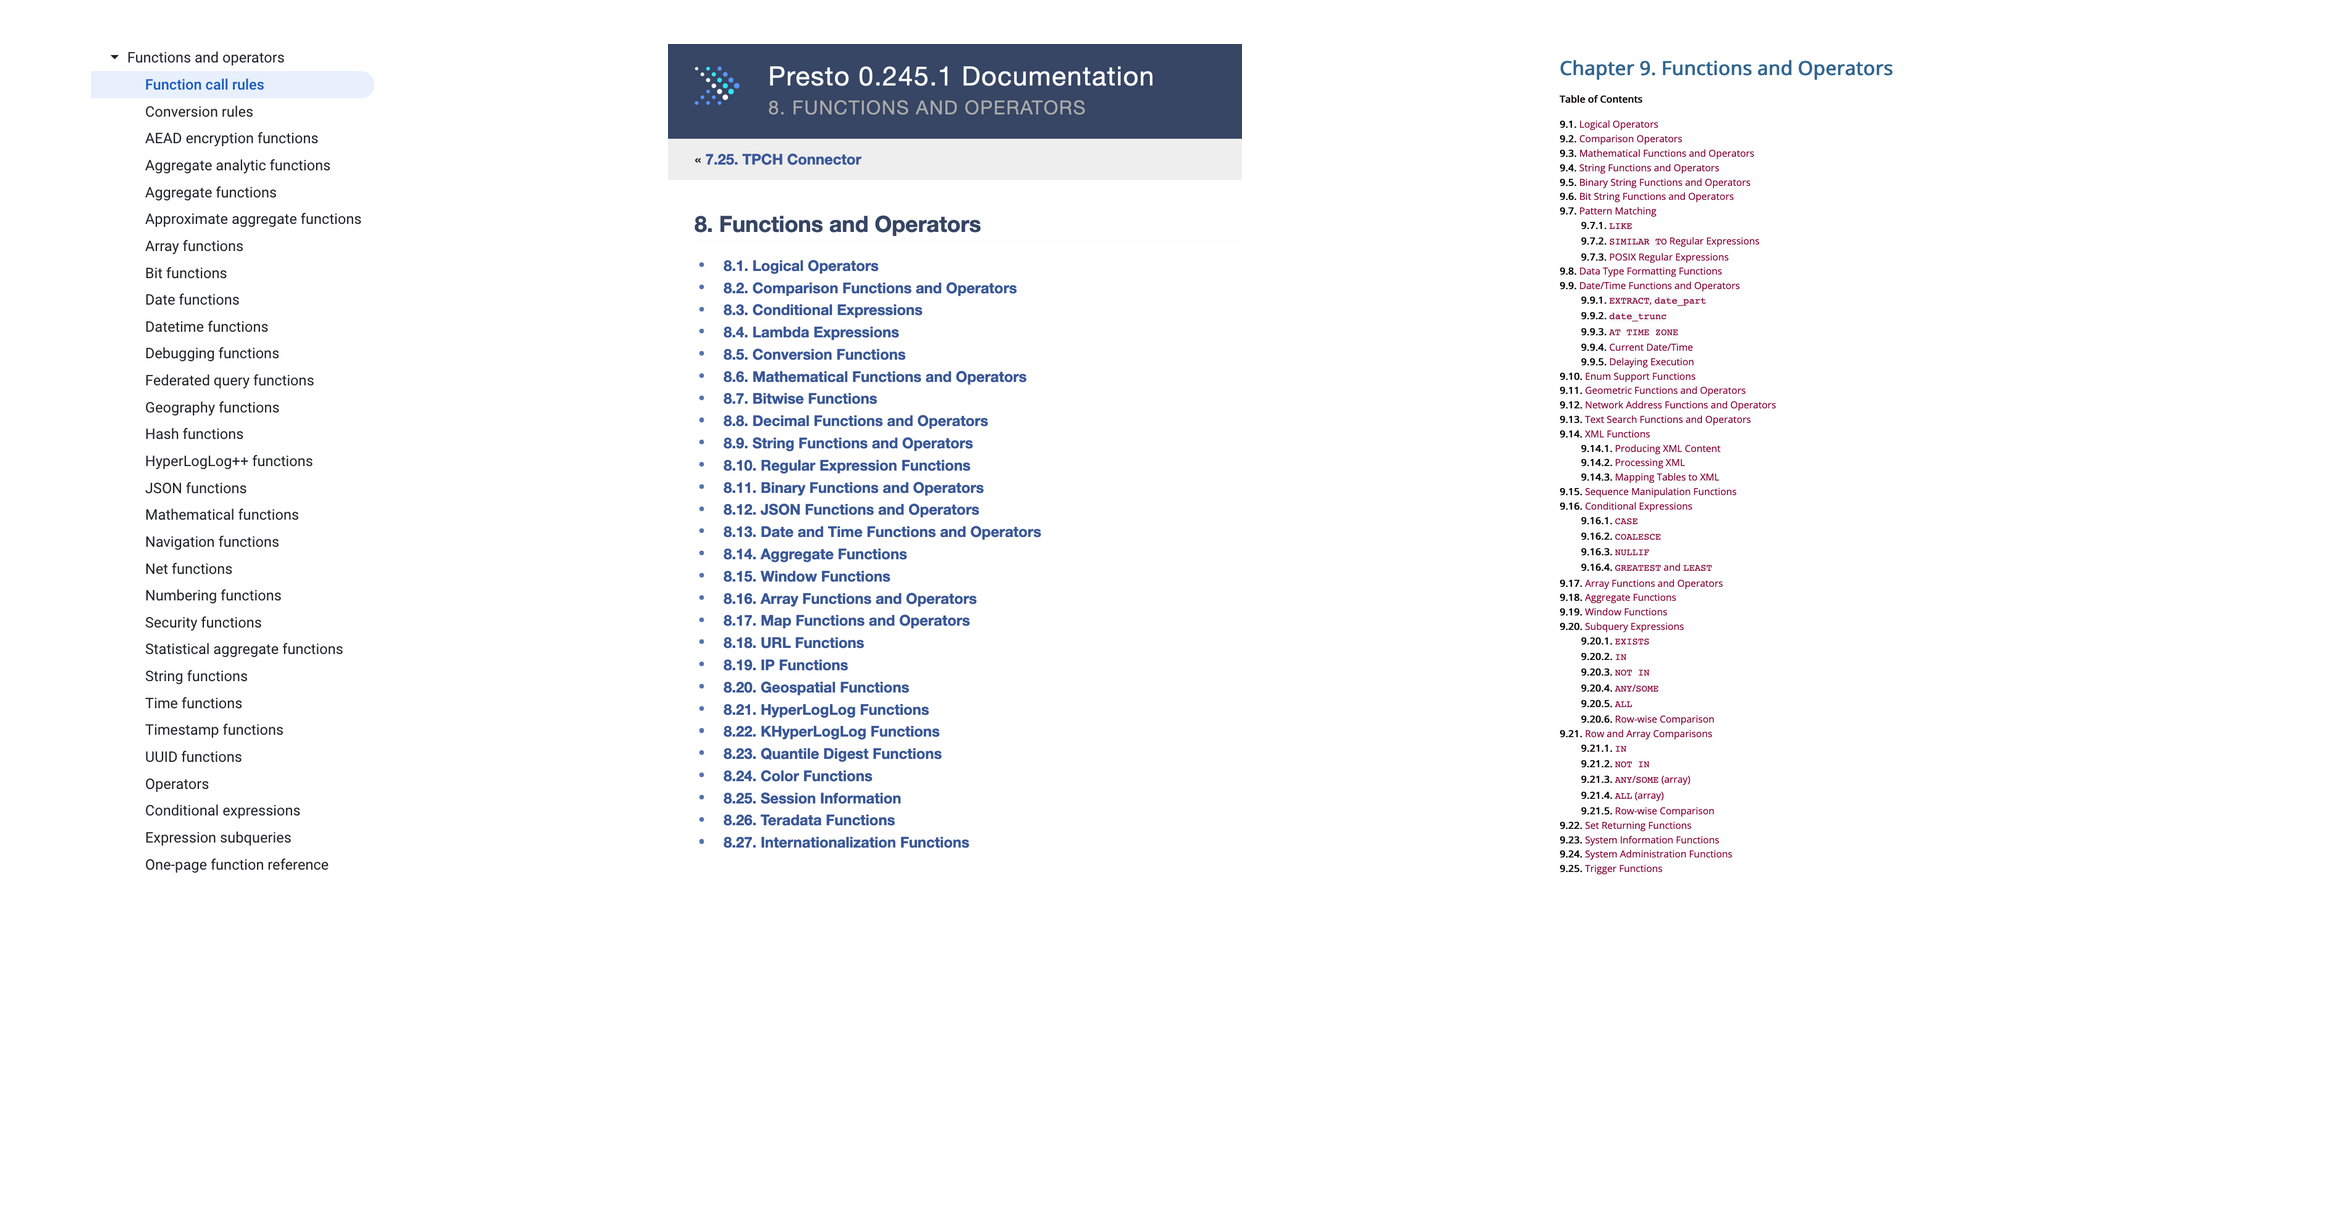
\includegraphics[height=.7\textheight]{udfs_all}
\end{frame}

\begin{frame}{Can call other services}
AWS Aurora allows to call AWS SageMaker\footnote{scalable backend that serves custom Machine Learning containers, basically any Python/R/etc. model even with Pytorch even on GPU!} directly

\begin{mdframed}[style=codeframe]\inputminted{sql}{aws-aurora-sagemaker.sql}\end{mdframed}
\end{frame}

\begin{frame}{And even more functionality}
Often SQL databases also provide ability to manage:

\begin{itemize}
    \item users and groups who can access database
    \item access control policies (ACL) to limit what users can see and modify
    \item triggers — functions to execute when events happen in database
    \item backups, migrations, connections to other databases, binlogs, ...
\end{itemize}
\end{frame}

\begin{frame}{Is the syntax the same everywhere?}
Notable differences between databases:

\begin{itemize}
    \item Advanced SQL like windows
    \item Different edge case handling
    \item User Defined Functions (UDFs)
    \item Unstructured data (JSON, XML)
    \item Types
    \item Aggregate functions, strings, special functions
    \item Triggers, Constants, Access Control Policies
    \item Transactions
    \item Partitions
    \item Indexes
\end{itemize}
\end{frame}

\begin{frame}{How to access database? Where do you input SQL?}
CLI, DataGrip, MySQL Workbench, BigQuery, Zeppelin, Jupyter, Tableau, and many more tools.. or from your programming language

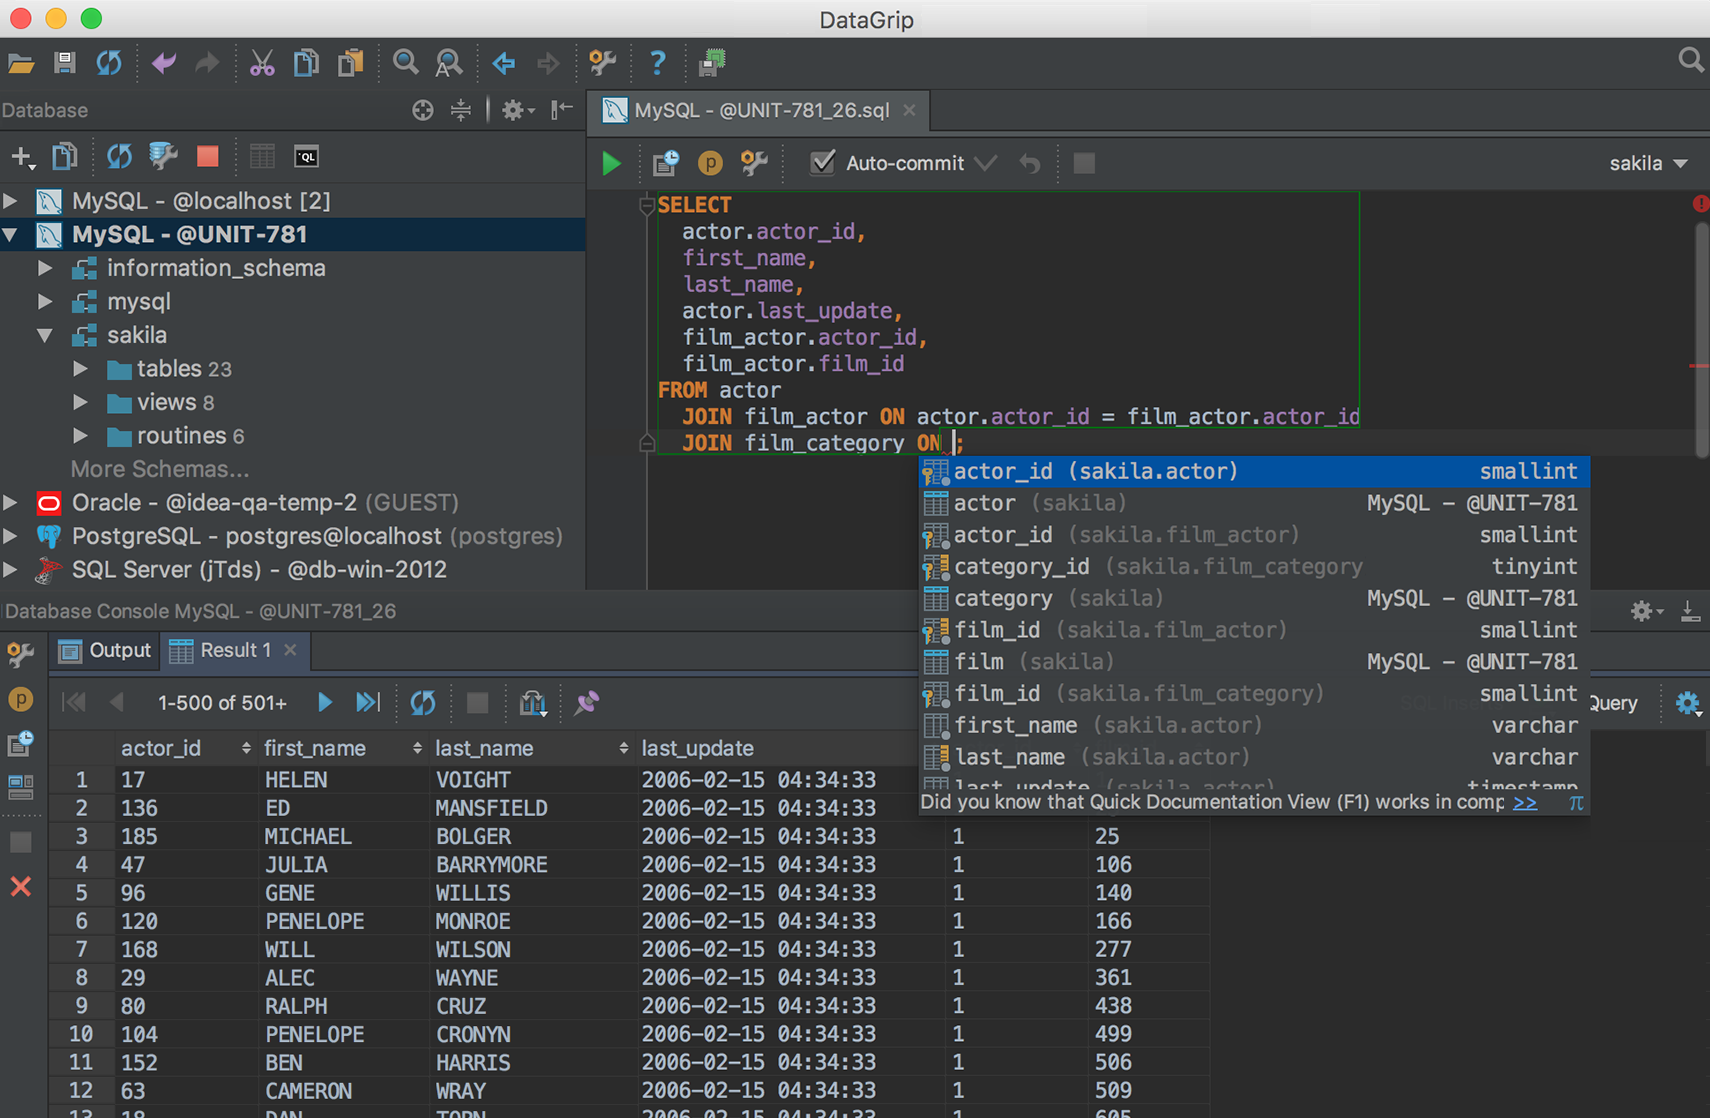
\includegraphics[height=.22\textheight]{example-datagrip}
\includegraphics[height=.22\textheight]{example-mysql}
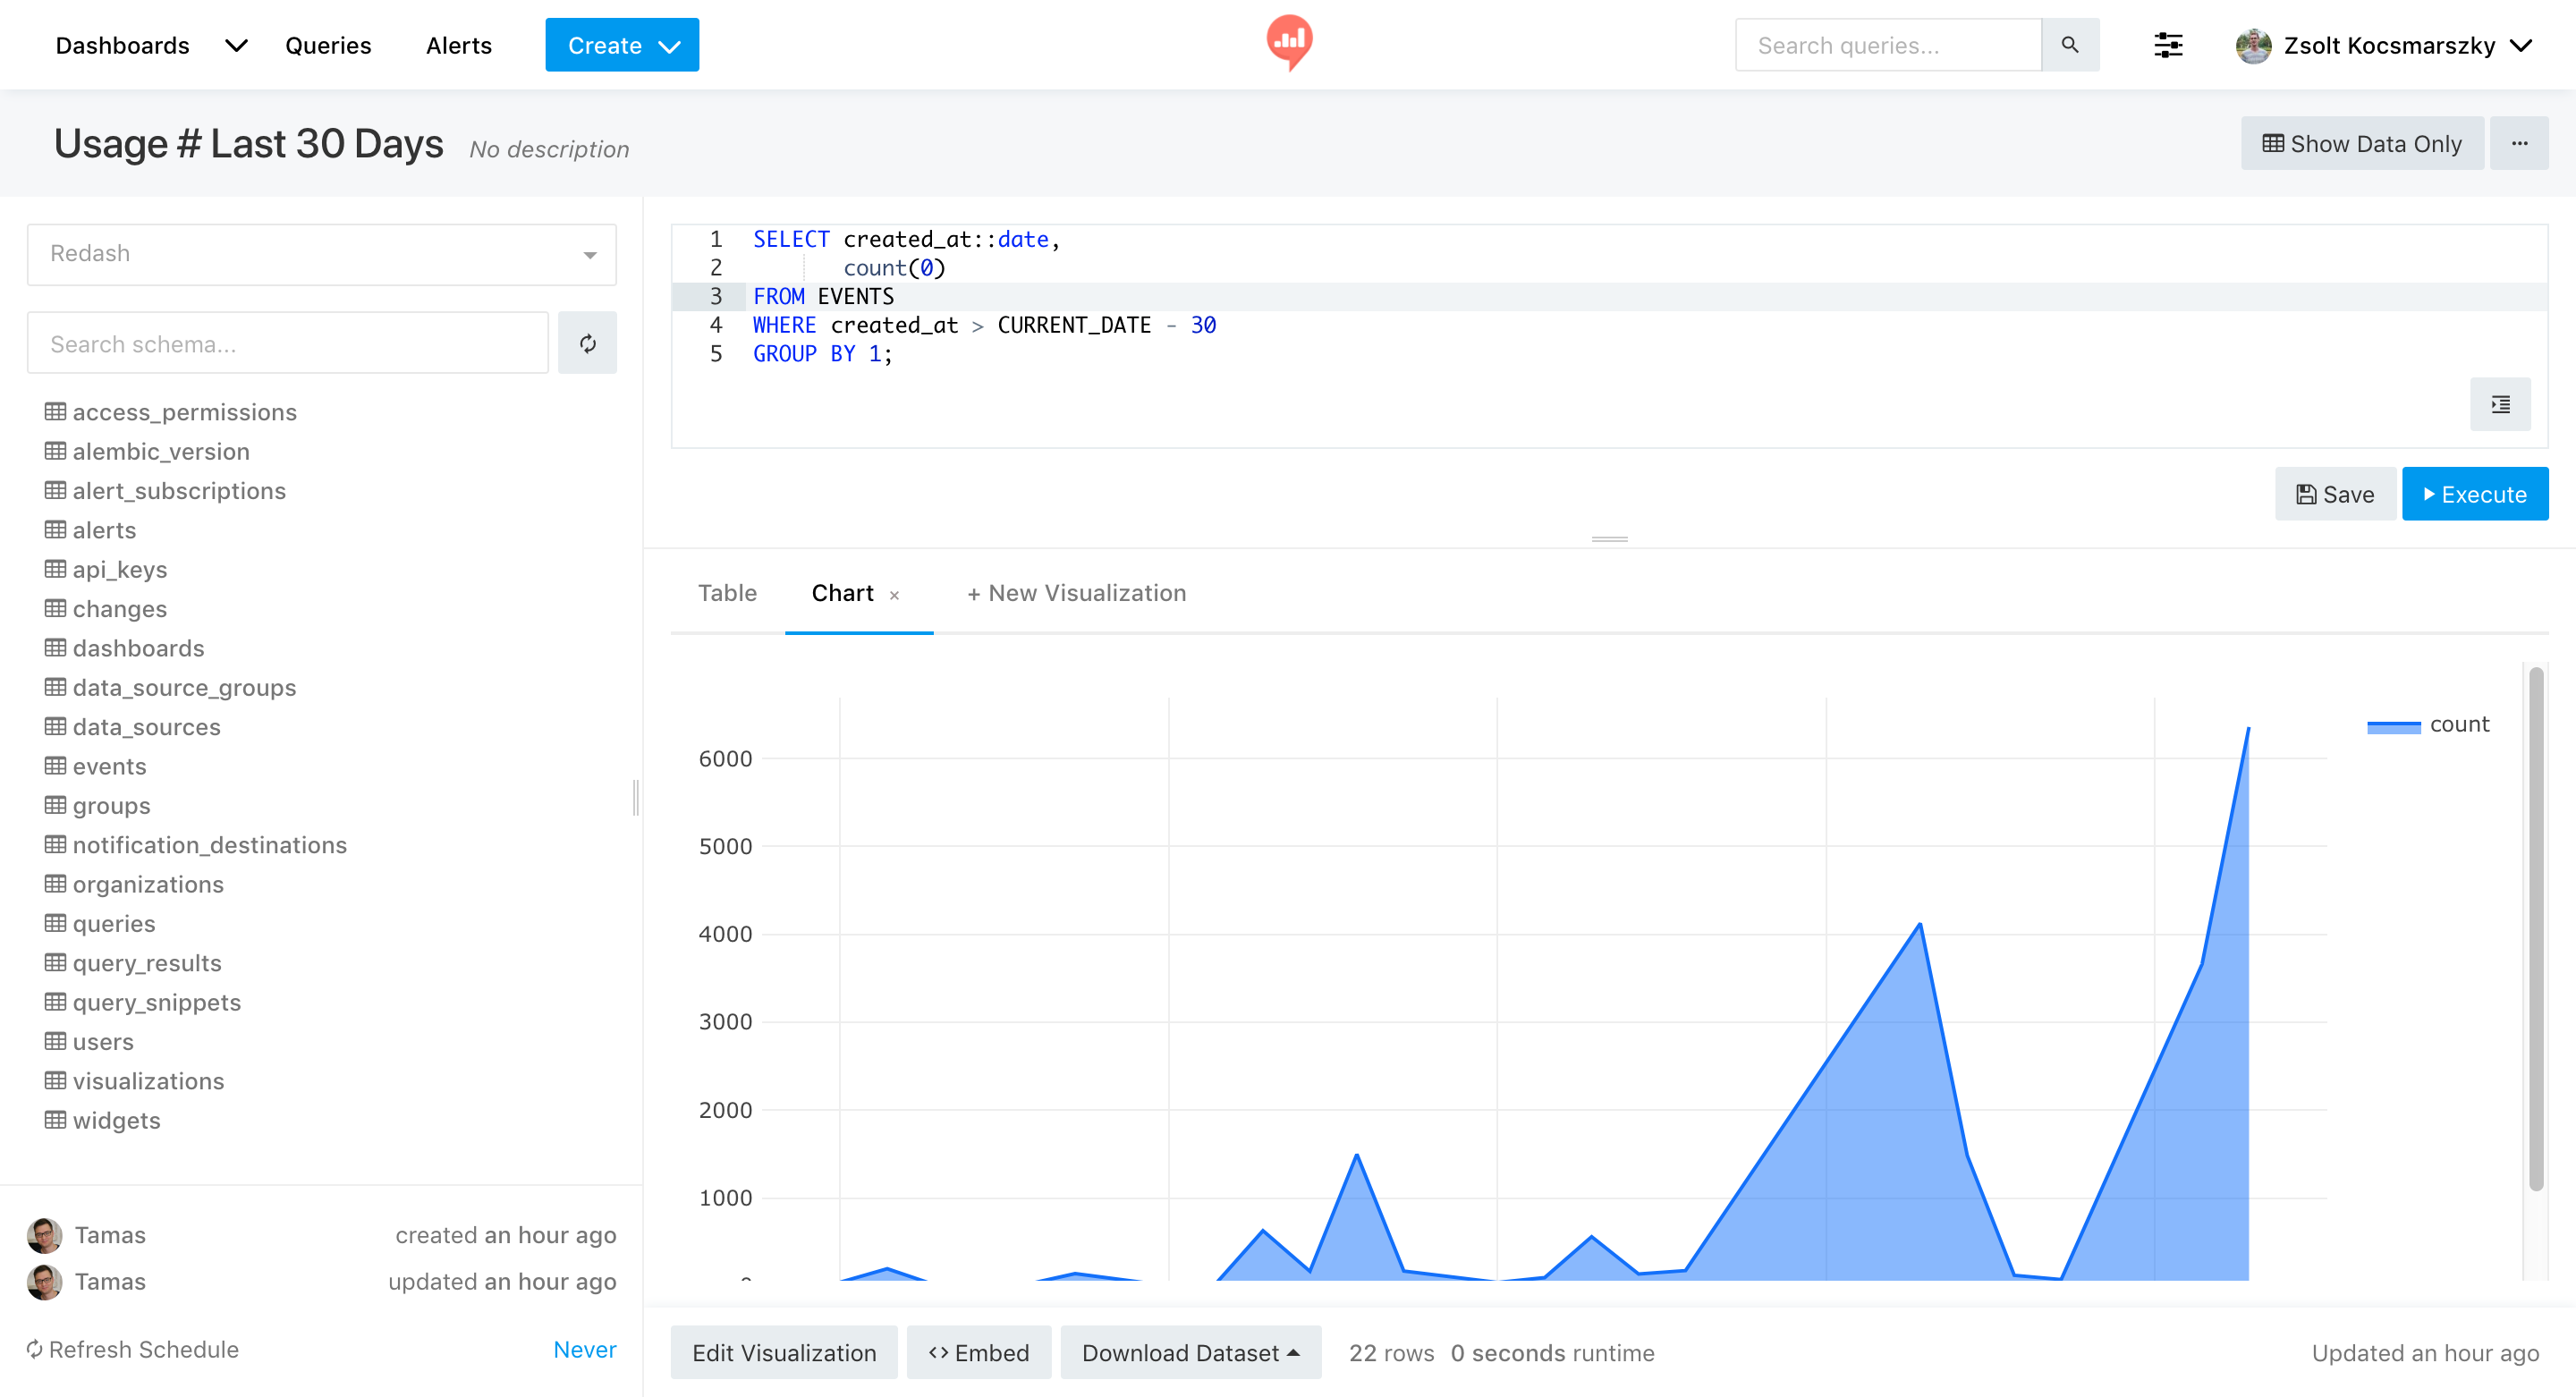
\includegraphics[height=.22\textheight]{example-bigquery}
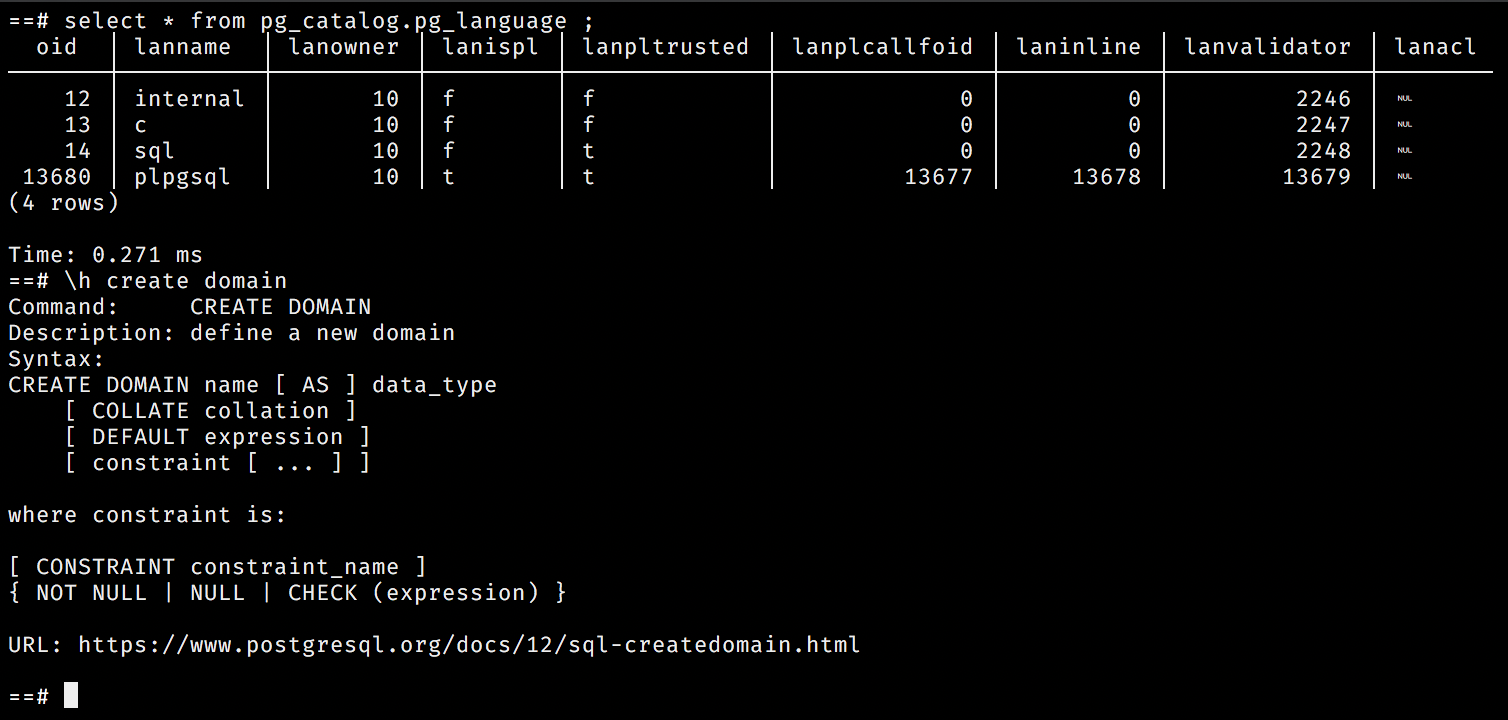
\includegraphics[height=.22\textheight]{example-psql}
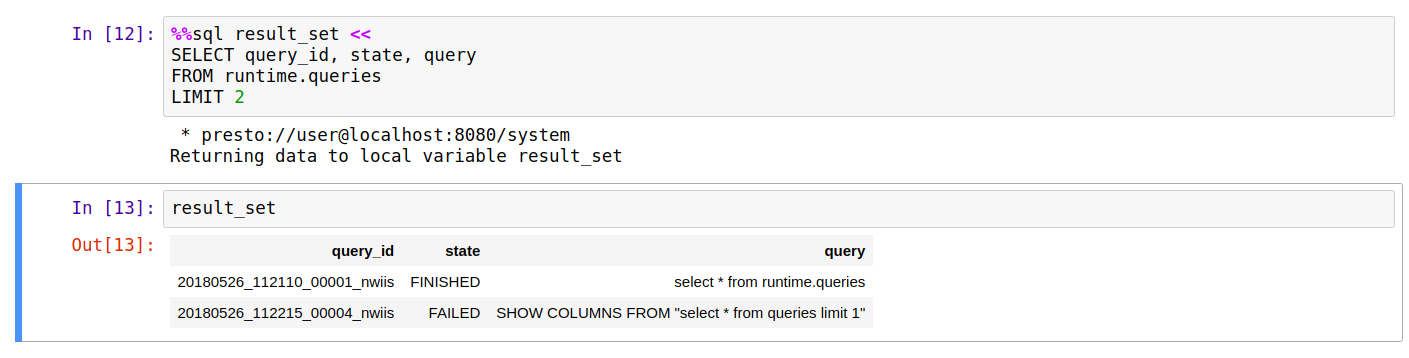
\includegraphics[height=.22\textheight]{example-jupyter}

\end{frame}

\begin{frame}{Common patterns for programmatic access}
\begin{itemize}
    \item Create Read Update Delete entity management (CRUD)
    \item Object Relational Mapping (ORM)
    \item Frequently updated data (e.g. counters)
    \item Infrequently updated data (e.g. employees)
    \item Event logs (e.g. iOS or Android app events) 
    \item Business Intelligence (BI) dashboards (e.g. Tableau)
    \item Machine Learning feature processing (Feature Store)
\end{itemize}
\end{frame}

\section{Database Internals}
\begin{frame}{Taxonomy of SQL databases}

Over time more hand-tailored solutions appear for each domain

\begin{center}
SQL
\end{center}

\begin{columns}
\begin{column}{0.3\textwidth}
    \begin{center}
    OLTP
    \end{center}
    \begin{itemize}
        \item MySQL
        \item PostgreSQL
        \item Oracle
        \item Aurora
        \item ...
    \end{itemize}
\end{column}
\begin{column}{0.3\textwidth}
    \begin{center}
    OLAP
    \end{center}
    \begin{itemize}
        \item BigQuery
        \item Spark
        \item Presto
        \item Hive
        \item Redshift
        \item ...
    \end{itemize}
\end{column}
\begin{column}{0.3\textwidth}
    \begin{center}
    Other
    \end{center}
    \begin{itemize}
        \item Timescaledb
        \item kdb+
        \item ...
    \end{itemize}
\end{column}
\end{columns}
\end{frame}

\begin{frame}{OLTP: Online Transactions Processing}
\begin{quote}
Money transfer between two specific people in bank that is happening right now
\end{quote}

Characterised by:
\begin{itemize}
   \item ultra-low latency
   \item updates and removals
   \item integrity
   \item simple queries
   \item indexes
   \item infra never fails
\end{itemize}

Examples: MySQL, PostgreSQL, Oracle, Microsoft SQL Server
\end{frame}

\begin{frame}{OLTP}
\begin{quote}
How does OLTP achieve its goals?
\end{quote}

\begin{itemize}
    \item indexes — quickly find out where data is located
    \item replication — if one node fails, then fallback to others, and improve read queries
    \item partitioning — to increase number of connections and parallelism
    \item multi-tier data storage — avoiding data loss
    \item snapshots, backups, logs — to avoid data loss
\end{itemize}

\end{frame}

\begin{frame}{OLAP: Online Analytics Processing}
\begin{quote}
Aggregate statistics on money transfers over hundreds of millions of people over twenty years
\end{quote}

Characterised by:
\begin{itemize}
    \item ultra-high throughput
    \item read-only
    \item complex queries
    \item partitions
    \item infra can fail
    \item idempotentcy
\end{itemize}

Examples: Hive, Spark, Presto, Redsfhit, BigQuery, Athena
\end{frame}

\begin{frame}{OLAP}
\begin{quote}
How does OLAP achieve its goals?
\end{quote}

\begin{itemize}
    \item partitioning — to increase parallelism
    \item avoiding shuffles — to decrease communication
    \item encourage idempotency — safe to restart processing
\end{itemize}
\end{frame}

\begin{frame}{Other domains}
... and there are much more

\begin{itemize}
    \item \textbf{TimescaleDB} for timeseries for analytics, IoT
    \item \textbf{kdb+} for high frequency trading, timeseries in finance
    \item .. and many other tools like \textbf{osquery} by Facebook to query status of corporate devices 
    \item .. and many connectors, even to crypto with \textbf{presto-ethereum}
\end{itemize}
\end{frame}

\begin{frame}{Other domains}
\begin{quote}
How do other databases achieve their design goals?
\end{quote}

Some common recurring themes:
\begin{itemize}
    \item partitioning
    \item replication
    \item caching
    \item query optimization
    \item heuristics of data and kinds of queries
    \item good utilization of OS and hardware
\end{itemize}
\end{frame}

\begin{frame}{Case study: Facebook}
\begin{itemize}
    \item OLTP — posts, users information, comments, and pretty much everything you see on Facebook is backed by one big MySQL\footnote{2018}
    \item OLAP — to do world-scale analytics for ads, integrity, business Facebook developed Hive and then Presto\footnote{2020}[]
\end{itemize}

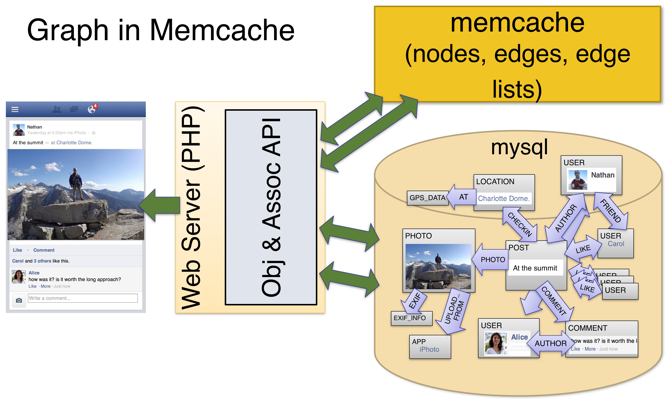
\includegraphics[height=.3\textheight]{example-fb-tao}
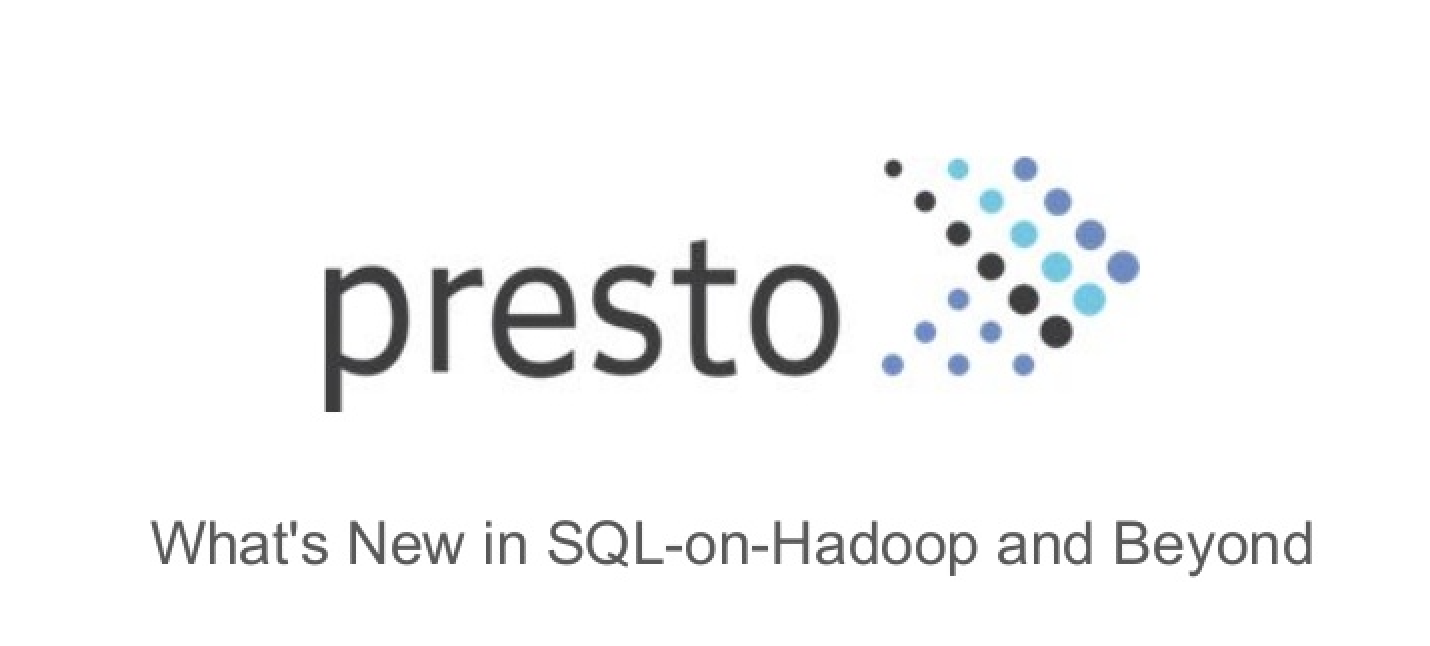
\includegraphics[height=.3\textheight]{example-fb-presto}

\end{frame}

\begin{frame}{Case study: Buzzfeed Machine Learning}
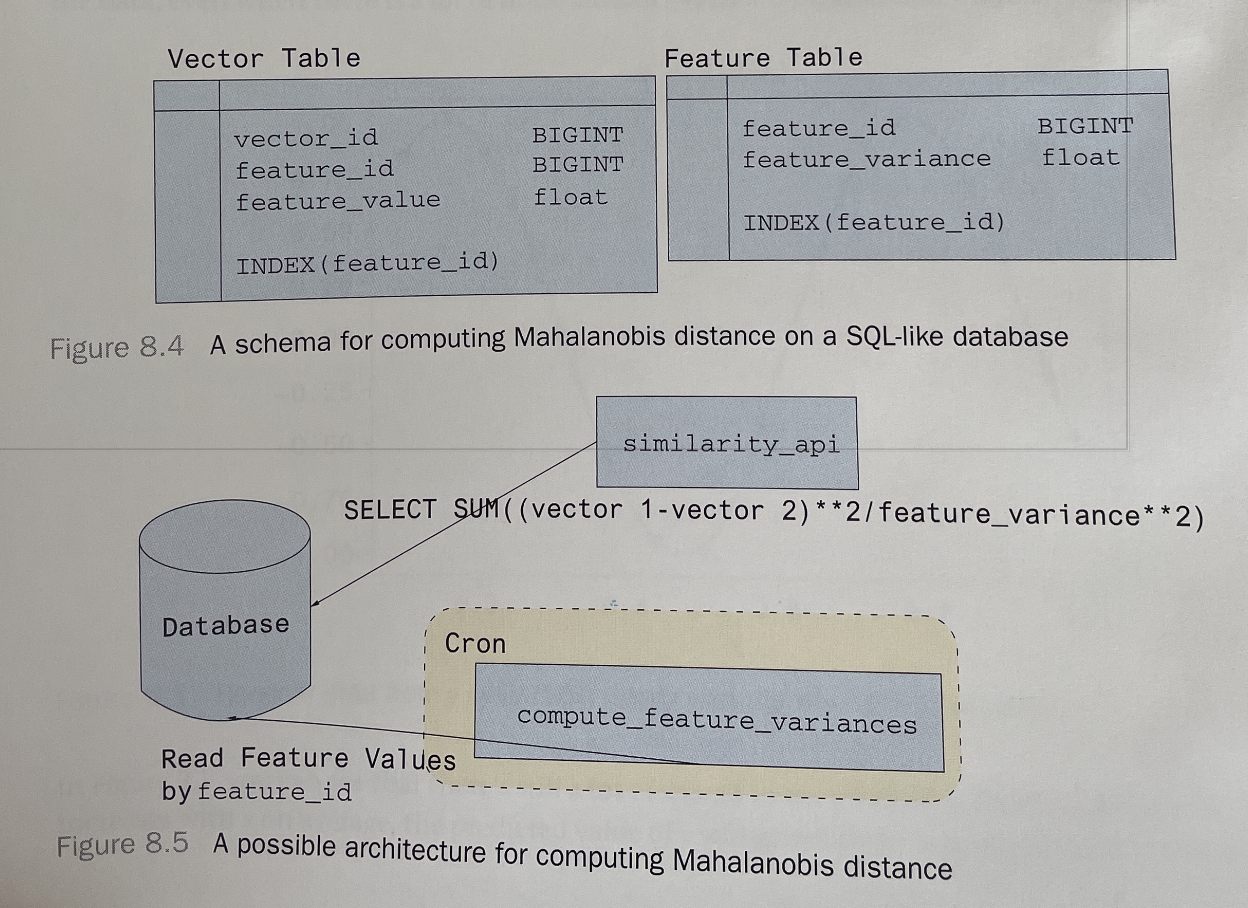
\includegraphics[height=.7\textheight]{buzzfeed_ml}
\end{frame}

\begin{frame}{Case study: Foodpanda, FSMK, Balancehero, Enswers, ...}

Pretty much any bank, government, airlines, or start-up is likely to be using SQL

\begin{itemize}
    \item OLTP — relational data is handled by backend team who likely to run typically either MySQL or PostgreSQL
    \item OLAP — analytics and machine learning is handled by data engineers, data scientists, business analysts, researchers who run either Spark, Presto, BigQuery, Athena, Tableau
\end{itemize}
\end{frame}

\begin{frame}{So how does it run exactly?}
\textbf{Single} node runs a process that accepts connections and spawns other worker process or thread per connection. Worker keeps some structures in memory, some on disk, smart query optimizer, lots of logic for resiliency and/or speed. Typically it is high-performance language like C or C++, but many OLAP databases are in Java.
\end{frame}

\begin{frame}{So how does it run exactly .. on a cluster?}
\textbf{Cluster} is multiple nodes that communicate over network. Typically it is a single master with multiple workers. Master receives queries from user, analyses it, creates execution plan and forwards work to workers. Alternatively, workers can just be a copy of master and serve read queries and master accepts writes.
\end{frame}

\section{Database Operations}

\begin{frame}{Self-hosted}
\begin{itemize}
    \item many databases are open-source and you can run it on your own hardware or EC2 instances, but you would have to manage \textit{backups, security, load balancing, networking, access, authentication, fail-overs, infrastructure automation, monitoring, alarms, compliance}
    \item some systems run tiny versions of SQL on device itself (e.g. SQLite inside iPhone)
\end{itemize}
\end{frame}

\begin{frame}{Cloud}
.. great power and great operational responsibility
\begin{itemize}
    \item OLTP: AWS Relational Database Service (RDS)
    \item OLAP: AWS EMR (Spark, Presto), Redsfhit
\end{itemize}

.. less power and less management overhead
\begin{itemize}
    \item OLTP: AWS Aurora
    \item OLAP: AWS Athena, GCP BigQuery
\end{itemize}
\end{frame}

\section{Further Study}

\begin{frame}{Further Study}
\begin{itemize}
    \item \textit{"Mastering PostgreSQL 12"}, Pakt
    \item \textit{"Designing Data Intensive Applications"}, O'Reilly
    \item \textit{"Expert Hadoop Administration"}, Addison-Wesley
    \item \textit{"The Data Warehouse Toolkit"}, Ralph Kimball 
    \item \textit{"Presto: SQL on Everything"}, Facebook original whitepaper
    \item Certifications \textit{AWS Data Analytics, AWS Database, GCP Data Engineer}
    \item .. and so much more
\end{itemize}
\end{frame}

\begin{frame}{Thank you!}
\begin{center}
github.com/nikolaydubina
\end{center}
\end{frame}

\end{document}